\documentclass[border=10pt]{standalone}

\usepackage{tikz}
\usepackage{tikzsymbols}
\usetikzlibrary{calc,patterns,shapes.geometric}

\def\centerarc[#1](#2)(#3:#4:#5){\draw[#1] ($(#2)+({#5*cos(#3)},{#5*sin(#3)})$) arc (#3:#4:#5);}

\begin{document}
	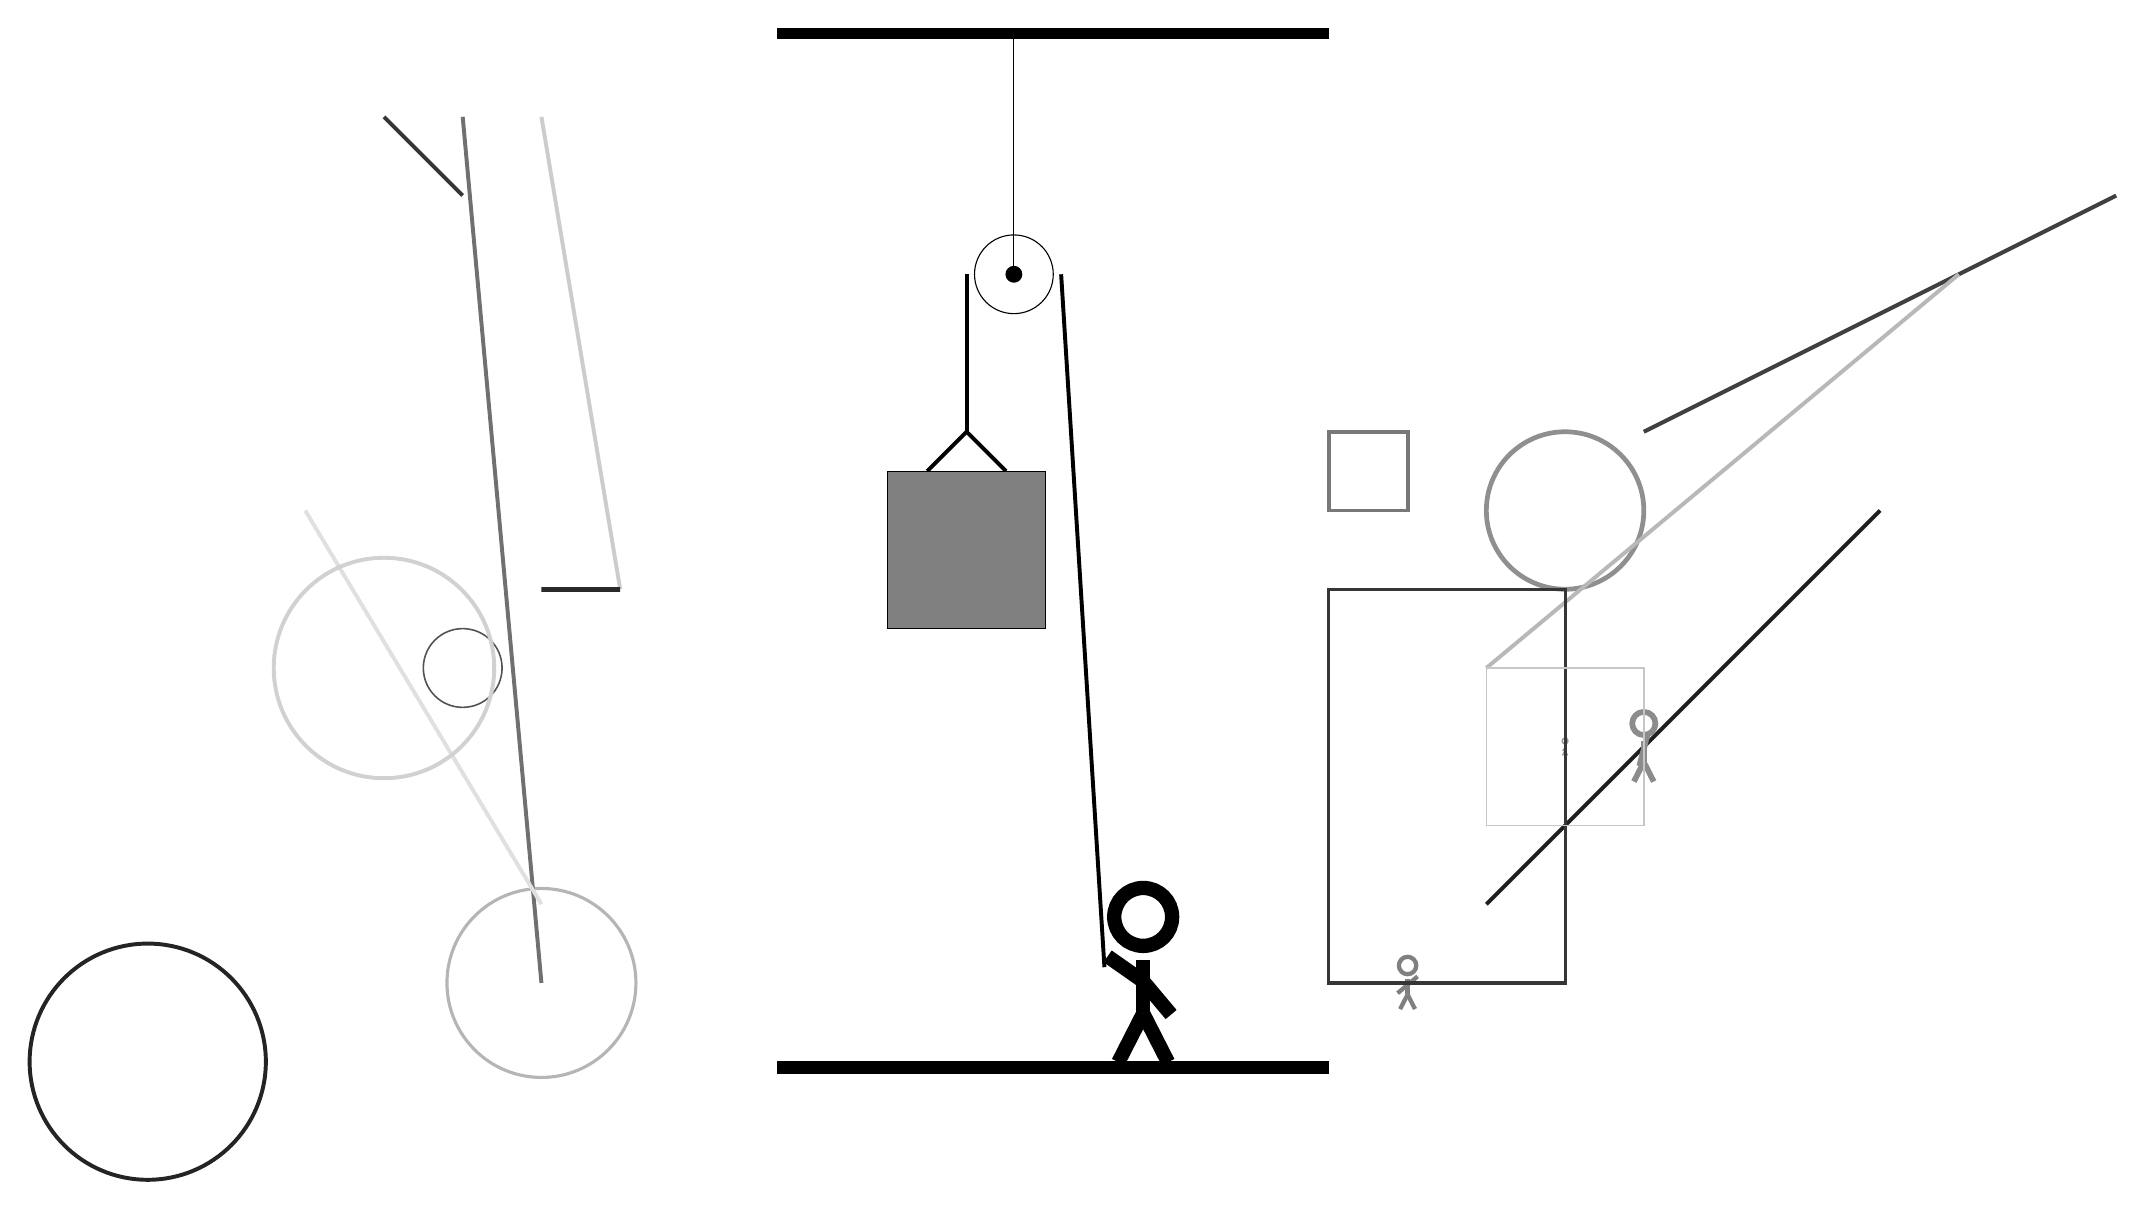
\begin{tikzpicture}
		%%%%% START %%%%%
		
		\draw[fill=black] (-2, 10) rectangle (5, 10.125);
		
		\draw (1, 7) circle (0.5);
		\draw[fill=black] (1, 7) circle (0.1);
		\draw (1, 10) -- (1, 7);
		
		\draw[line width=0.5mm] (-0.1, 4.5) -- (0.4, 5.0) -- (0.9, 4.5);
		\draw[fill=black!50] (-0.6, 4.5) rectangle (1.4, 2.5);
		
		\draw[line width=0.5mm] (0.4, 7) -- (0.4, 5.0);
		\centerarc[line width=0.5mm](1, 7)(0:180:0.6);
		\draw[line width=0.5mm](1.6, 7) -- (2.15, -1.8);
		
		\draw[line width=0.5mm, color=black!79](-6, 8) -- (-7, 9);
		
		\draw [line width=0.4mm, color=black!29](-5, -2) circle (1.2);
		\draw [line width=0.6mm, color=black!44](8, 4) circle (1.0);
		\draw [line width=0.2mm, color=black!95](12, 5) circle (0.0);
		\draw[line width=0.5mm, color=black!20](-5, 9) -- (-4, 3);
		\draw[line width=0.5mm, color=black!75](9, 5) -- (15, 8);
		\draw[line width=0.5mm, color=black!88](7, -1) -- (12, 4);
		
		\draw [line width=0.2mm, color=black!68](-6, 2) circle (0.5);
		\node[line width=0.5mm, color=black!45] at (9, 1) {\Strichmaxerl[4][75][76]};
		\node[line width=0.3mm, color=black!50] at (6, -2) {\Strichmaxerl[3][40][40]};
		\node[line width=0.5mm, color=black!41] at (8, 1) {\Strichmaxerl[1][58][86]};
		\draw[line width=0.5mm, color=black!28](7, 2) -- (13, 7);
		\draw[line width=0.6mm, color=black!84] (-4, 3) rectangle (-5, 3);
		
		\draw[line width=0.5mm, color=black!53] (6, 4) rectangle (5, 5);
		\draw[line width=0.5mm, color=black!56](-6, 9) -- (-5, -2);
		\draw[line width=0.4mm, color=black!79] (5, 3) rectangle (8, -2);
		\draw [line width=0.5mm, color=black!86](-10, -3) circle (1.5);
		\draw[line width=0.5mm, color=black!12](-5, -1) -- (-8, 4);
		\draw[line width=0.2mm, color=black!22] (7, 2) rectangle (9, 0);
		\draw [line width=0.5mm, color=black!18](-7, 2) circle (1.4);
		
		\node at (2.6, -1.9) {\Strichmaxerl[10][-35][-50]};
		
		\draw[fill=black] (-2, -3) rectangle (5, -3.15);
		
		%%%%% END %%%%%
	\end{tikzpicture}
\end{document}